%begin-include

In this section we provide the concepts that are fundamental to 
understand the biological and computational problems, methodologies and
results that we will present in this work. We start this chapter 
presenting what is a cell signaling pathway and how can one take 
measures to identify its activity on the cell. Later we present how 
it is possible to represent chemical iteractions as differential 
equations, and how that allows one to model a cell signaling pathway
with a system of ordinary differential equations. Then, we present 
more formally the problem we are trying to solve on this project, the
identification of cell signaling pathways, as well as the state of the
art methods of model ranking. Finally, we present the basics of 
posterior distribution sampling, which is a useful tool when working 
with Bayesian approaches, such as the ones used on this project to rank 
models.

% What I want to talk about in this section?
% - Cells signaling pathways are part of the cell communication system,
% and it allows the cell to perceive the conditions of the environment 
% and also to change its behaviour according to the input signal.
% - The signals perceived by a cell can come from cells that very close
% (including itself), as in synapses or it can travel long distances in 
% the organism, as in hormones.
% - When a signal reaches a cell, it can either activate a receptor in
% the cell membrane or diffuse into the cell.
% - Once this happen, the signal or the activated receptor can trigger
% a sequence of chemical interaction, altering the conformation and 
% state of proteins and also changing the concentration of chemical 
% species in the cell. Ultimately, this chain of effects can alter the 
% behaviour of the cell, what is called signal transduction.
% - Studying signaling pathways is important because they help us 
% understand the mechanisms of a cell, which can for example, elucidate 
% treatments for diseases.
\section{Cell Signaling Pathways}
Cell signaling pathways are part of the complex cell communication 
system, and it allows the cell to perceive the conditions of the 
environment in which it is placed and change its behaviour accordingly.
Signaling pathways participate in the regulation of many cell functions,
including development, division and cell death~\cite{Hancock2017}. The
dynamic of a signaling pathway can also be releated to diseases, as in
many cases of cancer.

The signal perceived by a cell can come from cells that are close 
(including the same cell that produced the signal), as in synapses, or 
it can travel long distances in the organism, as in hormones. When a 
signal reaches a cell, it binds to a specific receptor in the membrane,
and once that happens, the receptor can trigger a sequence of chemical 
interactions that can include change of conformation of proteins, 
activation or inactivation of proteins, and change of concentration of
chemical species in the cell. Ultimately, this chain of chemical 
reactions caused by the signal can alter the behaviour of the cell, what 
is called signal transduction.

Since signaling pathways participate in many of the cell functions, and 
are also related to diseases, it is important to study those structures
in order to get a better understanding of the cell mechanisms and 
diseases. One approach on the study of the cell signaling pathways is to 
measure the concentration change of proteins and how they interact to
produce those changes.

% - Western blot is a technique that can indicate the amount of a 
% specific protein that is in a mixture of proteins
% - This technique shows the presence of a protein in a mixture by 
% ``blotting'' these molecules into a membrane. 
% - Repeating the procedure in different times define time-course 
% observations of the protein in a biological experiment.
% - With these observations in hand, the researcher is able to construct 
% a measurement that is relevant to describe the biological experiment. 
% For instance, in a signaling network where a protein is closely 
% related to the behaviour of interest of the cell, this protein is a 
% good candidate as a measure of the system.
\section{Measurements of Proteins in Cell Signaling Pathways}
Western blot~\cite{Towbin1979} is a laboratory technique that can 
indicate the amount of a specific protein that is present in a mixture. 
This technique shows the presence of a protein in a mixture by 
``blotting'' a membrane where the molecules of interest are located. We 
can summarize the procedure in the following steps: first a mixture 
containing a sample of cells of interest must be created; 
second, proteins from the mixture should be fixed on the blotting 
membrane; third, an antibody should bind to the target protein 
molecules; and finally, a method for highlighting the bound antibody 
should be applied. An image of the resulting membrane can then be 
analyzed with computer programs to quantify the relative concentration 
(with respect to some other protein, usually a control protein that has 
fairly the same concentration during the whole experiment) of the 
protein of interest.

By repeating this procedure in different times it is possible to create 
time-course observations of proteins throughout the biological 
experiment. With this tool, a researcher can choose a set of relevant 
proteins from a signaling network and gain knowledge about the dynamics 
of such chemical species during the experiment. For instance, in a 
signaling network experiment in which it is desired to understand how
the change of concentrations of a species at the beginning of the 
pathway changes the concentration of some species at the end of the 
cascade, then measurements of both are relevant to understand the 
biological experiment. Figure~\ref{fig:western_blot_example} presents an 
example of time-course Western blot for an experiment where it is 
desirable to understand how extracellular signal-regulated kinase (ERK)
is activated (phosphorylated) as a function of levels of Rat sarcoma
bound to guanosine triphosphate (Ras-GTP).

\begin{figure}[!ht]
\centering
    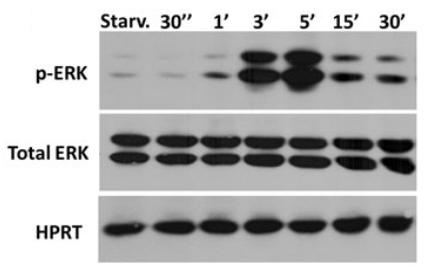
\includegraphics[width=\textwidth]{fundamental_concepts/western_blot.png}
    \caption{Figure {\bf a} shows time-course measurements of ERK, 
    phosphorylated ERK (p-ERK) and hypoxanthine-guanine 
    phosphoribosyltransferase (HPRT). HPRT is a ``loading'' protein, 
    that means that its concentration is fairly the same through the 
    experiment, and therefore it is used as a normalizing factor to 
    total ERK concentration. Figure  {\bf b} shows values of 
    phosphorylated ERK that are obtained after processing Figure 
    {\bf a}. Original image of Marcelo S. Reis et al. 
    (2017)~\cite{Reis2017}.}
    \label{fig:western_blot_example}
\end{figure}

These measurements alone do not always provide means for researchers to 
understand a cell signaling pathway experiment. However, if we create a 
computational model for this signaling networks that is able to 
reproduce experimental data, then we might use this model as a 
summary of the signaling network, which can provide to researchers 
evidences of the biological phenomena.


% What do I need to talk about?
% - We can model the concentration changes of chemical species as 
% differential equations, using the mass-action kinetic laws
% - The mass action kinetic law states that in an elementary reaction,
% the rate of a chemical reaction is directly proportional to the 
% product of the reactants concentrations.
% - What is elementary?
% 2.1 Elementary reactions rate equations
% - Types of elementary: first order reaction and second order reaction
% - How do we write up these two? 
% - Chemical notation with constants
% - From there we can write a system of differential equations to 
% describe the signaling pathway.
% - As an example, let's show the equations for a simple enzymatic 
% equation.
% 2.2 Simplifications of reactions
% - More can be done. We can simplify some equations 
% 2.1 Mass conservation simplification
% 2.2
\section{Dynamic Modeling of Cell Signaling Pathways}
One approach onto modeling cell signaling pathways is to model the 
dynamics of the concentrations of chemical species involved. This can be
accomplished when using the law of mass action~\cite{Voet2010}. This law 
states that, in an elementary reaction, the speed (or rate) of a 
chemical reaction is proportional to the product of the concentration of 
all reactants. An elementary reaction is a reaction in which there is no 
participation or need of an intermediate reaction to describe the first 
in a molecular level. In practice, it is more common to see two types of 
elementary reactions, they are first or second order reactions. 

\subsection{Modeling Elementary Reaction Rates}
A first order reaction is composed of one reactant only. Suppose A is 
the only reactant and B is the only product of a reaction, then we can
write this reaction as:
\begin{equation*}
\ce{
    A -> B
}.
\end{equation*}
The reaction rate of this reaction, according to the law of mass 
action, is 
\begin{equation*}
    k_1[\text{A}],
\end{equation*}
where $k_1$ is some constant and [A] is the concentration of A. It is
import to note that the constant $k_1$ is a rate coefficient of the 
reaction and, therefore, it can only assume positive values.

A second order reaction is composed of two reactants. Suppose C and D 
are both and the only reactants and F is the product of a reaction, then
we can write this reaction as:
\begin{equation*}
\ce{
    C + D -> F
}.
\end{equation*}
The reaction rate of this reaction is
\begin{equation*}
    k_2\text{[C][D]},
\end{equation*}
where $k_2$ is a (positive) constant and [C] and [D] are the 
concentrations of C and D, respectively.

Using these two laws to calculate the speed of reactions, we are able 
to describe how the concentration of chemical species in a system change 
through time using differential equations. To illustrate this and future 
concepts of this section, we are going to consider a minimal system 
composed of a simple enzymatic reaction:
\begin{equation}
\ce{
    E + S <=>[\ce{$k$_f}][\ce{$k$_r}] ES ->[\ce{$k_{cat}$}] E + P
},
\label{eq:simple_enzymatic}
\end{equation}
where E is an enzyme, S is a substrate, ES is the enzyme-substrate
complex, and P is the product.

Each arrow in Equation~\ref{eq:simple_enzymatic} represents one 
elementary reaction, and the names over or under arrows represent 
reaction rate constants. All three reactions can be represented by the
equations:

%The first reaction has E and S as reactants and
%ES as a product, and can be written as 
\begin{subequations}
\begin{align}
\ce{
    E + S ->[\ce{$k_f$}] ES 
} \label{eq:es_complex_fwd} \\
\ce{
    ES ->[$k_r$] E + S
} \label{eq:es_complex_rev} \\
\ce{
    ES ->[$k_{cat}$] E + P
} \label{eq:es_pe} 
\end{align}
\end{subequations}
and they have, respectively, reaction rates of:
\begin{equation*}
\begin{aligned}
    & k_f\text{[E][S]} \\
    & k_r\text{[ES]} \\
    & k_{cat}\text{[ES]}.
\end{aligned}
\end{equation*}

Now, to determine a model of the concentration dynamics for
Reaction~\ref{eq:simple_enzymatic}, we will write a system of ordinary
differential equations. To do so, we should take every chemical species 
and calculate its concentration change rate based on the rate of each 
reaction that it participates. For instance, the enzyme E is a 
reactant on Reaction~\ref{eq:es_complex_fwd} and is also a product on 
reactions~\ref{eq:es_complex_rev} and~\ref{eq:es_pe}, then we consider 
that E changes its concentration over time ($t$) according to the 
differential equation:
\begin{equation}
    \frac{d[\text{E}]}{dt} = -k_f\text{[E][S]} + (k_r + k_{cat}) \text{[ES]}
\end{equation} 
Note that we are adding reation rates in which the species is a product
and we are subtracting reaction rates in which the species is a
reactant. Repeating this procedure for every other species of the 
enzymatic reaction leads to the following system of ordinary 
differential equations:
\begin{subequations}
    \label{eq:full_system}
    \begin{align}
        \frac{d[\text{E}]}{dt} & =  
            -k_f\text{[E][S]} + (k_r + k_{cat}) \text{[ES]} 
            \label{eq:dEdt} \\
        \frac{d[\text{S}]}{dt}  & = 
            -k_f\text{[E][S]} + k_r\text{[ES]} 
            \label{eq:dSdt} \\
        \frac{d[\text{ES}]}{dt} & =  
            k_f\text{[E][S]} - (k_r + k_{cat}) \text{[ES]} 
            \label{eq:dESdt} \\
        \frac{d[\text{P}]}{dt} & = k_{cat}\text{[ES]} \label{eq:dPdt}.
    \end{align}
\end{subequations}

% Ok, what do I really want to talk about here: Michaelis Menten 
% simplification of enzymtic reactions
% - Before anything, we should use mass conservation to produce the 
% d[ES]/dt equation.
% - Then we should mention the steady-state proposal of Michaelis Menten
%   -> should I use a picture? Maybe I can compare two initial states,
%      one with [S] >> [E] and the other not.
% - Mention that we can suppress a lot of parameters with this 
%   simplification
\subsection{Simplification of Dynamic Models}
The System~\ref{eq:full_system} can be simplified if we
apply properties of enzymatic reactions together with algebraic 
simplifications. We will show then how to derive the quasi-steady-state 
Michaelis-Menten model for enzymatic reactions. With the correct 
assumptions, this model is able to reproduce the behaviour of an 
enzymatic reaction without considering the intermediate enzyme-substrate 
complex, leading to simpler models.

A basic principle we need to apply to our system in order to derive
the Michaelis-Menten model is the principle of mass conservation. This 
principle is valid if we assume that the 
reactions~\ref{eq:simple_enzymatic} are isolated, meaning that the 
chemicals on these reactions are not involved in other reactions at the
same time. Applying this principle to the enzyme chemical, produces the
following equation:
\begin{equation*}
    \text{[E$_0$]} = \text{[E] + [ES]}.
    \label{eq:E_conservation}
\end{equation*}
If we apply this equation to the derivative of the concentration of ES,
we will get the following equation:
\begin{equation}
    \frac{d[\text{ES}]}{dt} =  
        k_f(\text{[E$_0$]} - \text{[ES]})\text{[S]} 
        - (k_r + k_{cat}) \text{[ES]}. 
        \label{eq:dESdt_2}
\end{equation}

One more assumption is necessary to derive the simplification. This 
assumption states that the concentration of substrate-enzyme complex
does not change over time, i.e. $\frac{d[\text{ES}]}{dt} = 0$, and it 
was first proposed in 1925 by Briggs and Haldane~\cite{Briggs1925}. 
Generally, this assumption is applicable whenever [S] $\gg$ [E]. 
If we apply this assumption together with the mass conservation 
assumption on the Equation~\ref{eq:dESdt_2}, we get:
\begin{equation*}  
    \begin{aligned}
        \text{[ES]} (k_r + k_{cat}) &= 
            k_f(\text{[E$_0$]} - \text{[ES]})\text{[S]}, \\
        \text{[ES]} &= \frac{\text{[E]}_0\text{[S]}}{K_m + \text{[S]}}, 
    \end{aligned}
\end{equation*}
in which $K_m = \frac{k_{cat} + k_r}{k_f}$ is known as Michaelis 
constant. Considering this, we can rewrite the rate of [P] as:
\begin{equation}
    \frac{d\text{[P]}}{dt} = k_{cat}\frac{\text{[E]}_0\text{[S]}}
        {K_m + \text{[S]}}.
    \label{eq:dPdt_2}
\end{equation}
And finally, if we apply mass conservation to the substrate, we will get
the following equation:
\begin{equation*}
    \text{[S$_0$]} = \text{[S] + [ES] + [P]},
\end{equation*}
then, we can differentiate this equation on $t$ and use the 
quasi-steady-state assumption ($\frac{d\text{[ES]}}{dt} = 0$) to obtain:
\begin{equation}
    \frac{d\text{[S]}}{dt} = - \frac{d\text{[P]}}{dt}.
    \label{eq:dSdt_2}
\end{equation}

Now, with equations~\ref{eq:dPdt_2}~and~\ref{eq:dSdt_2} we are able to
reproduce the dynamics of the substrate and product of the enzymatic 
reaction. Therefore, using the Michaelis-Menten model, we could simplify 
the System\ref{eq:full_system} that had four equations and three 
parameters to a new model that has only two equations and two parameters 
($k_{cat}$ and $K_m$). Figure~\ref{fig:michaelis_menten} shows a 
comparison between the dynamics of the complete and Michaelis-Menten 
models of enzymatic reactions.

\begin{figure}[H]
  \centering 
  \begin{tabular}{c c}
    \subfigure[] {\scalebox{1}{
    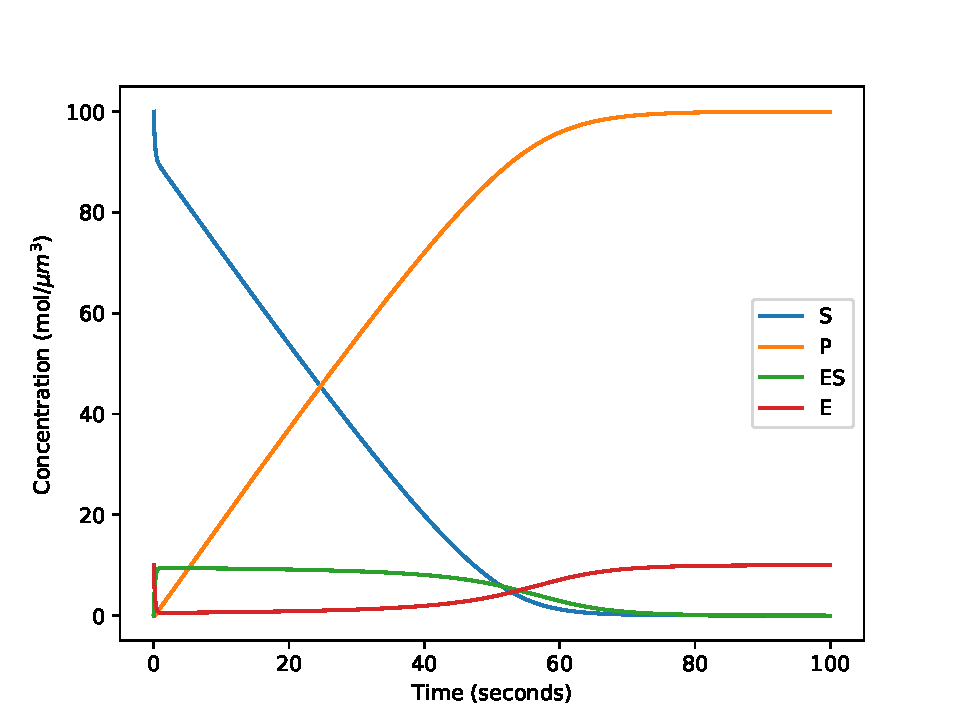
\includegraphics[trim={0 0 0 1.4cm}, clip=true, width=.45\textwidth]{fundamental_concepts/simplifications/full_system.pdf}}
     \label{fig:enzymatic_full}}
     &
    \subfigure[] {\scalebox{1}{
    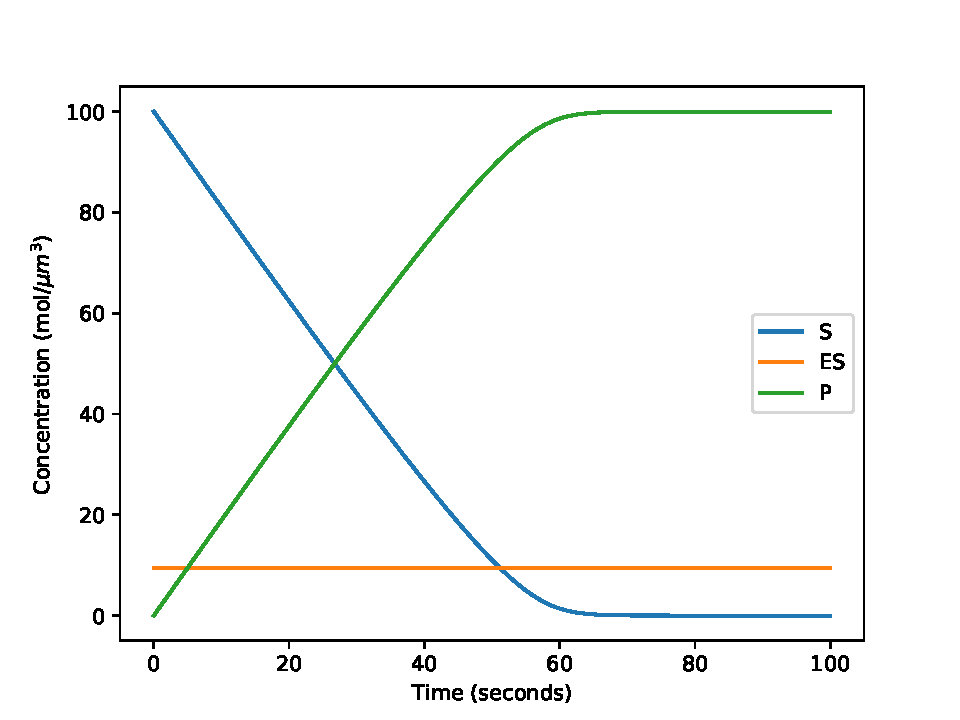
\includegraphics[trim={0 0 0 1.4cm}, clip=true, width=.45\textwidth]{fundamental_concepts/simplifications/mm_system.pdf}}
    \label{fig:enzymatic_mm}}
  \end{tabular}
    \caption{An example of the dynamics produced by two models of 
        enzymatic reactions. The Figure~\ref{fig:enzymatic_full} 
        presents the dynamics of the model~\ref{eq:full_system} and 
        Figure~\ref{fig:enzymatic_mm} presents the dynamics of the 
        Michaelis-Menten simplification to the same model. For this 
        simulations, it is necessary to define initial concentrations of
        the chemical species involved, and it is used: 
        10 molecules$/(\mu m)^3$ for the enzyme (E); 
        100~molecules$/(\mu m)^3$ is used for the substrate (S); and 
        0~molecules$/(\mu m)^3$ is used for the other species. In 
        addition to this, it is also necessary to define model 
        parameter values, and it is used: 
        0.06~$(\mu m)^3$(molecules$*s)^{-1}$ for $k_f$; 
        0.1~$(s^{-1})$ for $k_r$; 0.2~($s^{-1}$) for $k_{cat}$; and,
        following the Michalis-Menten model, 5 molecules$/(\mu m)^3$
        is used for $K_m$.}
  \label{fig:michaelis_menten} 
\end{figure}

% What to talk about:
% 1. Define identification of cell signaling pathways
%    -> Identification of signaling pathways is the problem of finding 
%       the components of a signaling network and how they interact 
%       in order to reproduce some behaviour of the cell that was
%       previously measured experimentally. 
%    -> The input of the problem should be then a description of the 
%       biological experiment and the measurements made on this 
%       experiment. As an output, we are expected to give a topology
%       of the network of interactions that are actively controlling
%       the cell behaviour observed on experiment measurements. More 
%       than that, we are also supposed to determine the set of 
%       parameter values that should be used on the models to reproduce
%       measurements similar to the experiments (or a probability 
%       distribution).
%    -> Two main tasks onto creating the output: you have to find 
%       a topology that is good with some parameter to reproduce the 
%       experiment; note that these tasks are very strongly correlated
%       and should be done together. 
% 2. Explain the challenges of cell signaling pathways
%    -> Firstly, simulating these problems is very time-consuming (even 
%       tough there are many ode solvers out there)
%    -> The number of possible interactions is very big. If we consider
%       choosing from n interactions a subset of them that should be on 
%       the topology, then there are 2^n options.
%    -> Once you choose two candidates of topology, it is still hard to
%       tell which one is better.
% (?). Talk about the work of Marcelo. State that current solutions do
%       not systematically search for the solution. 
% 3. somehow link to the next section, about cost functions 
%    -> Many of the state of the art approaches on identification of 
%       cell signaling network are based on a Bayesian approach for 
%       model ranking.
\section{Identification of Cell Signaling Pathways}
Identification of signaling pathways is the problem of finding the 
components of a signaling pathway and how they interact in order to
reproduce a cell behaviour that has been previously measured 
experimentally. The input of this problem is usually a description of 
the biological experiment, containing previous information about the 
signaling pathway, such as known reactions and parameters, and a set of 
measurements, commonly Western blot data, which is the only type of
measurement we consider in this work. The output to this problem is then
composed of a set of interactions that are actively controlling the
behaviour of interest of the cell, and also the set of parameter values 
that should be used on these interactions to create a model that
approximates the experimental observations; it is possible to output a
single value for each parameter, as it was presented in~\cite{Wu15}, or
output information about these values, using a posterior (to the
experimental data) distribution, as it was presented
in~\cite{Liepe2014}~and~\cite{Xura20}.

Two main tasks must be completed to produce such output. The first task
is to find candidate topologies for the pathway model, i.e. different
set of interactions that are relevant to the pathway of interest. The
second task is to rank those models according to their ability to 
simulate the pathway, approximating the experimental measurements.

% To the second task, you can use combinatorics optimization to fit the
% model to the data and calculate the distance of the measurements on 
% the fitted model to the experimental data; then it is possible to rank
% models according to this distance. Alternatively, it is 
% possible to consider that the model parameters are random variables 
% and calculate the marginal probability of the model to reproduce the 
% observed data; then, it is possible to rank models according to this 
% probability.

The second task is also known as the model selection problem and even
though it is a broad area, there are works on the literature that treat 
specifically the problem in a biochemical context. Solutions to this 
problem should be able to choose model candidates according to their 
ability to reproduce observed data, penalizing overly complex models 
to avoid overfitting. 

One approach on setting the score of a model is to search for the set of 
parameter values that make the model measurements the closest to the 
experimental data, and then define a distance between these two 
measurements; then it is possible to use this distance, plus a penalty 
for complexity, to create a ranking of the models. Note that a penalty 
function is needed because complex and more general models can overfit,
producing models that cannot represent the same signaling network with
small perturbations to biological experiment. We can write this scoring 
function as:
\begin{equation*}
    score_1 (M) = - min_{\{{\boldsymbol \theta} \in \Theta' \subset
        \Theta\}} dist (\phi(M, {\bm \theta}), {\bm D}) + R (M),
\end{equation*}
where $M$ is the model, $\Theta$ is the parameter space for model $M$, 
$\Theta'$ is the subset of the parameter space where the search for the
best parameter values was conduced, ${\bm D}$ is a list of experiment
measurement (each measurement is a time-course observation of the
biological phenomena of interest), $\phi$ is a function that determines
the simulated measurement on the model, and $R$ is a regularization
function that penalizes model complexity. This approach was implemented
on the work of Lulu Wu~\cite{Wu15}, using a Simulated Annealing
procedure to search for parameter values that minimize the distance
between simulation and experiment. The Simulated Annealing procedure
used is available on the software SigNetSim (Signaling Network
Simulator), which is based on the of the work of Chu on~\cite{Chu1999}.
However, Wu's methodology showed limitations when testing the ability to
reconstruct models from experiments, and this could be related to the
used penalization term. In fact, choosing a good regularization function
is crucial to the performance of this methodology.

Another approach to setting the model score is to consider the model 
parameters as random variables and then marginalize the probability of 
the model and parameters to reproduce the observed data, i.e. estimate 
(because calculating is usually hard) the marginal probability:
\begin{equation}
    p ({\bm D} | M) = \int_{\Theta} p ({\bm D} | M, {\bm \theta}) 
        p({\bm \theta} | M) d{\bm \theta},
    \label{eq:marginal_likelihood_integral}
\end{equation}
where ${\bm D}$ is the observed data, $M$ is the model and $\Theta$ is 
the parameter space for model $M$. The function $p({\bm \theta} | M)$ is 
the prior probability function of the parameter ${\bm \theta}$ on model 
$M$. The function $p ({\bm D} | M, {\bm \theta})$ is the likelihood of 
observing the data ${\bm D}$ when simulating the model $M$ using 
parameters $\theta$. Sometimes, however, the likelihood function is 
unknown or computationally intractable; for these cases, it is possible 
to use an alternative Bayesian approach, called Aproximate Bayesian 
Computation (ABC), to estimate the probability $p (M | {\bm D})$ and use 
it as a ranking score~\cite{Toni2009}.

% However, to the first task, there are not many methods on the 
% literature to solve this problem. Generally, this is solved using 
% both interactome maps from KEGG and the prior knowledge of the 
% researchers.
For the first task of identification of signaling pathways we described
(the creation of model candidates), there are not as many works on the 
literature as there are for the second task. Commonly, researchers must 
resort on their own knowledge on the biological experiment and consult 
interactome maps available on repositories such as KEGG and BioModels to
construct manually the hypothesis of models for a signaling pathway. 
That enlightens the importance to create a methodology that 
systematically creates candidate models of signaling networks, as we 
propose on this project.



% What are the best approaches on model selection recently
% -> Most of them uses Bayesian ideas
% -> good because they can provide statistical formality about the 
%    selection.
% -> automatic penalization; allows researcher to introduce biological
%    information through the priors.
% -> it makes sense that a parameter is a random variable
% -> Explain BIBm
% -> Explain ABC-SysBio
% -> Even though they provide ways of ranking models, they don't treat
% the modeling of the network topology.
% -> Bayesian approaches
\section{State of the Art in Selection of Biochemical Models}
The state of the art in biochemical model selection is based on Bayesian
inference. The Bayesian approaches provide the benefits of ranking 
models with statistical formalism, and automatically penalizes overly 
complex models. More than that, through the prior distribution of the
parameters, the researcher is able to input prior knowledge about 
interactions constants; this type of information can facilitate the 
parameter inference of models since it tends to concentrate the search.

Bayesian approaches consider that model parameters are random variables, 
instead of fixed unknown constants. We can argue that this modeling is 
fair to the reality in biochemical processes because interactions 
constants can vary depending on the cell conditions. Therefore, in a 
biological experiment in which there might be perturbations to the cell 
environment, it should be more adequate to rank models integrating the 
models score over a probability space of parameters instead of fitting 
the model to data using a single point of the parameter space. We will 
now present the basic concept of two methods that use this idea for 
model selection, the Annealing-Melting Integration 
(AMI)~\cite{Vyshemirsky2007} and Approximate Bayesian Computation 
(ABC)~\cite{Toni2009}.

% What to mention about AMI:
% -> thermodynamic integral
% -> we are estimating the log of p(D|M, theta)
% -> theta being distributed according to some q_beta (\theta)
% -> q_beta are bridging distributions from prior to posterior
% -> to estimate this integral we need to use Monte Carlo Markov Chains
The Annealing-Melting Integration is a method that estimates the 
integral~\ref{eq:marginal_likelihood_integral} using concepts of 
thermodynamics. With thermodynamic integration, it is possible to write 
the logarithm of this integral as:
\begin{equation}
    \ln p({\bm D}|M) 
            = \int_0^1 \expectation_{q_\beta({\bm \theta})} 
              [\ln p({\bm D} | M, \theta)] d\beta
        \label{eq:thermodynamic_integral}
\end{equation}
where $p({\bm D}|M,\theta)$ is the likelihood function (the 
probability of observing the data ${\bm D}$ when $M$ is the correct
model, with parameters ${\bm \theta}$); and 
$\expectation_{q_\beta ({\bm \theta})}$ is an expectation taken over the 
probability space of 
$q_\beta({\bm \theta}) \propto 
p({\bm D}|M, {\bm \theta})^\beta p({\bm \theta}|M)$. The variable 
$\beta$ works in the integral as a temperature term, determining the 
probability functions $q_{\beta}({\bm \theta})$, $\beta \in [0, 1]$; 
note that when $\beta = 0$ then 
\begin{equation*}
q_0({\bm \theta}) = p({\bm \theta}|M),
\end{equation*}
the prior distribution of the parameters; also, and when 
$\beta = 1$ then 
\begin{equation*}
    q_1(\theta) = \frac{p({\bm D}, {\bm \theta}| M)} {\int_{\Theta}
                            p({\bm D}, {\bm \theta}| M)} 
                = \frac{p({\bm \theta} | {\bm D}, M)p({\bm D}|M)} 
                        {p({\bm D} | M)}
                = p({\bm \theta} | {\bm D}, M),
\end{equation*}
the posterior distribution of parameters. Therefore, the 
integral~\ref{eq:thermodynamic_integral} takes the expected value of the
likelihood function of ${\bm D}$ over a sequence of probability 
distributions that is a ``bridge of distributions'' connecting the prior
and posterior distributions of parameters. Calculating this integral is 
usually infeasible, hence in practice it is needed to estimate this 
integral using samples of a finite number of tempered distributions, 
$q_\beta({\bm \theta})$.

% How about ABC?
% -> Likelihood free!
% -> Define the algorithm
%   -> The goal of the algorithm is to find a ``good" sample of 
%      parameters for the observed data.
%   -> The algorithm proposes a candidate parameter \theta*.
%   -> Simulate the model with those parameters.
%   -> Using a distance function d, accept theta* if
%      d(simulation, data) < eps
As we mentioned before, the likelihood function 
$p({\bm D} | M, {\bm \theta})$ may be very hard to calculate if not 
impossible. For those cases it is possible to use a parameter inference
approach that is likelihood-free, called Approximate Bayesian 
Computation (ABC). This method has the goal of producing a sample of 
parameters that brings the model simulations close to the observed data.
A generic ABC algorithm starts proposing a candidate parameter 
${\bm \theta}^*$ from a proposal distribution; then, a simulation, 
$\phi (M, {\bm \theta}^*)$ of the model using the candidate parameters
is produced; if, for some distance function $d$, it is true that 
$d(\phi(M, {\bm \theta}^*), {\bm D}) < \epsilon$, then we accept 
${\bm \theta}^*$ as part of the sample. If $\epsilon$ is sufficiently 
small, then the produced samples approximates well the posterior 
distribution. To use ABC methods for model selection it is enough to add
a model indicator parameter to the parameter array, then it is possible
to extract model distribution from the accepted parameters.

% Metropolis-Hastings algorithm
% -> Both methods for model selection, based on ABC or using 
% thermodynamics integration needs to generate samples of probability 
% distributions. Generating samples of distributions is easy for many 
% well known distributions, however, for some other distributions it may
% not simple. 
% -> What does it do?
% Metropolis-Hastings algorithms are capable of generating a
% sample that has some probability distribution $p$, the target 
% function. The method can be used even when it is not possible to 
% calculate points of the target probability function, because all it is
% needed is a function that is proportional to the target. This is 
% useful for example when the target function is a posterior
% -> How do we do this
%   -> 
\section{Metropolis-Hastings to Generate Samples}
Both methods for model selection, based on ABC or using thermodynamics
integration need to generate samples of probability distributions. 
Generating samples of distributions is simple for many well known 
distributions, however, for some other distributions it may not be as
simple. Metropolis-Hastings algorithms are capable of generating a 
sample that has some probability distribution $p$, which is called the 
target distribution. In fact, the method can be used even when it is not
possible to access directly the target function, because all it is 
needed to perform the sampling is a function that is proportional to the
target.

Being able to generate a sample of a target distribution without 
accessing the probability function itself is useful for our applications
in Bayesian model ranking. Consider that we need to create a sample of
the parameters posterior distribution $p (\theta | M, D)$. Calculating 
this probability function is very hard because
\begin{equation*}
    p(\theta | M, D) = \frac{p (D | \theta, M) p (\theta | M)}
                            {p (D|M)},
\end{equation*}
and this equation has the term $p (D|M)$, which is only known (by some 
estimation) at the end of the model ranking; however, if we can access
the likelihood function $p (D| \theta, M)$ and the prior 
$p (\theta | M)$ than the product of these two is proportional to the 
posterior distribution (since $p (D|M)$ is only a constant because it
does not depend on $\theta$), and therefore they are enough to generate
a sample of the posterior.

A generic Metropolis-Hastings algorithm that creates a sample of a 
target distribution $p (\lambda)$ proceeds as follows:
\begin{enumerate}
\item{Choose some starting point $\lambda_0$ for which $p (\lambda_0)$ 
    is not zero. Also set $t = 1$.}
\item{Sample a candidate point $\lambda^*$ from a proposal (or jumping) 
    distribution with probability $J_t (\lambda^* | \lambda^{t - 1})$.}
    \label{enum:iteration_start}
\item{Calculate the ratio:}
    \begin{equation}
        r = \frac{p (\lambda^*) J_t (\lambda^{t - 1} | \lambda^*)}
                 {p (\lambda^{t - 1}) J_t (\lambda^* | \lambda^{t - 1})}
        \label{eq:mh_ratio}
    \end{equation}
\item{With probability $min (1, r)$ set $\theta^t = \theta^*$ and set
    $\theta^t = \theta^{t - 1}$ otherwise.}
\item{Increase $t$ by one and, if not reached limit number of 
    iterations, go back to step~\ref{enum:iteration_start}.}
\end{enumerate}
Note that if the target $p (\lambda)$ is not available, and rather 
another function $q (\lambda) = \frac{1}{c}p(\lambda)$ is available, 
then the ratio~\ref{eq:mh_ratio} can be calculated as:
\begin{equation*}
    r = \frac{p (\lambda^*) J_t (\lambda^{t - 1} | \lambda^*)}
              {p (\lambda^{t - 1}) J_t (\lambda^* | \lambda^{t - 1})} 
      = \frac{(q (\lambda^*)c) J_t (\lambda^{t - 1} | \lambda^*)}
           {(q (\lambda^{t - 1})c) J_t (\lambda^* | \lambda^{t - 1})} 
      = \frac{q (\lambda^*) J_t (\lambda^{t - 1} | \lambda^*)}
              {q (\lambda^{t - 1}) J_t (\lambda^* | \lambda^{t - 1})}
\end{equation*}
More than that, if the proposal distribution is symmetric, the produced 
algorithm is called Metropolis algorithm and has the ratio 
$r = {p (\lambda^*)}/{p (\lambda^{t - 1})}$. 

Different implementations of the Metropolis-Hastings algorithm are 
possible. The possible changes include the choice of starting point,
the choice of proposal distributions and number of iterations. As an
example, some algorithms are adaptive in the sense that they can change 
the proposal distribution according to the acceptance rate of proposed 
points~\cite{Gelman2013}.
